%%%%%%%%%%%%%%%%%%%%%%%%%%%%%%%%%%%%%%%%%%%%%%%%%%%%%%%%%%%%%%%%%%%%%%%%%%%%%%%%%%%%%%%%%%%%%%%%%%%%%%
%%%%%%%%%%%%%%%%%%%%%%%%%%%%%%%%%%%%%%%%%%%%%%%%%%%%%%%%%%%%%%%%%%%%%%%%%%%%%%%%%%%%%%%%%%%%%%%%%%%%%%
%%%%                                                                                       %%%%%%%%%%%
%%%% Plantilla de trabajo de titulación para la Carrera de Ingeniería en Construcción -UCM %%%%%%%%%%%
%%%% Elaborada por Carlos Palacios Rojas, Académico Dep Obras Civiles                      %%%%%%%%%%%
%%%% Versión 1.2.1 - 12 de septiembre de 2016                                              %%%%%%%%%%%
%%%% Las líneas que comienzan por "%" son comentarios y pueden ser eliminadas.             %%%%%%%%%%%
%%%% En caso de requerir más información del uso de los paquetes buscar en Internet.       %%%%%%%%%%%
%%%%                                                                                       %%%%%%%%%%%
%%%% Recomiendo el siguiente libro para consultas sobre Latex                              %%%%%%%%%%%
%%%% Mora, W., & Borbón, A. (2014). Edición de textos cientıficos con LATEX. 2da edición.  %%%%%%%%%%%
%%%%																					   %%%%%%%%%%%
%%%%%%%%%%%%%%%%%%%%%%%%%%%%%%%%%%%%%%%%%%%%%%%%%%%%%%%%%%%%%%%%%%%%%%%%%%%%%%%%%%%%%%%%%%%%%%%%%%%%%%
%%%%%%%%%%%%%%%%%%%%%%%%%%%%%%%%%%%%%%%%%%%%%%%%%%%%%%%%%%%%%%%%%%%%%%%%%%%%%%%%%%%%%%%%%%%%%%%%%%%%%%


\documentclass[10pt,letterpaper]{report}

	% Geometry: es para modificar los márgenes del documento
\usepackage[left=3cm, right=2.5cm, top=2.5cm, bottom=2.5cm]{geometry}
%% lipsum: para generar texto de ejemplo. Se puede eliminar una vez que se eliminen todos los \lipsum[] del documento.
\usepackage{lipsum}
% lscape: en caso de querer rotar una hoja, buscar información en internet en caso de ser requerido. 
\usepackage{lscape}
% inputenc: para que latex acepte caracteres latinos como los acentos y la letra ñ.
\usepackage[utf8]{inputenc}
% babel: para traducir los títulos que vienen originalmente en inglés. Ejemplo: Fecha, Chapter, Bibliography, Appendix, etc.
\usepackage[spanish,es-tabla]{babel}
% natbib: para poder citar utilizando paréntesis redondos con \citep{•} o sin parentesis con \cite{•}
\usepackage[round]{natbib}
\usepackage{float} % para usar [H] y obligar que las figuras o tablas aparezcan donde es requerido.
\usepackage[pdftex]{graphicx} % graphicx: para incorporar imágenes. Recordar que las imágenes 'gif' no son aceptadas por Latex, se sugiere utilizar formato png por su calidad, en segunda intantcia jpg.
\usepackage{parskip} % parskip: par no dejar sangrías e insertar espacios entre párrafos en su lugar.
\usepackage{amsmath} %paquete para escribir fórmulas matemáticas.
\usepackage{amsfonts}%paquete para escribir fórmulas matemáticas.
\usepackage{amssymb} %paquete para escribir fórmulas matemáticas.
\usepackage[usenames,dvipsnames,svgnames,table]{xcolor} %xcolor: para definir colores y dar color a tablas.

% hyperref: define opciones especiales para el documento PDF producido.
\usepackage[pdftex, bookmarksnumbered,  pagebackref, colorlinks=true, citecolor=DarkBlue, linkcolor=DarkBlue!30!Black, urlcolor=Black,bookmarksopen]{hyperref}

% El paquete fancyhdr es para definir opciones de encabezado y pié de página
% Según el formato existente a la fecha (agosto de 2015) esto no se considera
% Su utilización en este caso es para situar el número de página en la parte
% inferior derecha de la página.

\usepackage{fancyhdr} % activamos el paquete
	\pagestyle{fancy} % seleccionamos un estilo
	\lhead{} % texto izquierda de la cabecera
	\chead{} % texto centro de la cabecera
	\rhead{\textcolor[gray]{0.5}{\textit{\nouppercase \leftmark}}} % Nombre del capítulo. \nouppercase: uso de minúsculas
	\lfoot{} % texto izquierda del pie
	\cfoot{} % imagen centro del pie
	\rfoot{\textcolor[gray]{0.5}{\thepage}} % Número de página a la derecha, abajo
	\renewcommand{\headrulewidth}{0.2pt} % grosor de la línea de la cabecera

\fancypagestyle{detailed}{
    \fancyhf{} % clear all header and footers
    \fancyfoot[R]{\textcolor[gray]{0.5}{\thepage}}
	%\fancyhead{}    
    \renewcommand{\headrulewidth}{0pt}
 }
 
\usepackage{etoolbox}
\patchcmd{\chapter}{\thispagestyle{plain}}{\thispagestyle{detailed}}{}{}

%times: para uar letra tipo Times New Roman
\usepackage{times}

%separación entre líneas (1.2 espacios). En word es interlineado exacto a 12 pts
\renewcommand{\baselinestretch}{1.2} 

\usepackage{titlesec} % para poder modificar los títulos

% Para la numeración de tablas y figuras.
\renewcommand\thefigure{\arabic{section}.\arabic{figure}} % Genera numeración X.Y
\renewcommand\thetable{\arabic{section}.\arabic{table}} % Genera numeración X.Y
\numberwithin{figure}{section} %Hace que la primera figura de cada sección X sea X.1
\numberwithin{table}{section} %Hace que la primera tabla de cada sección X sea X

\usepackage{booktabs} % Para trabajar con opciones especiales de tablas.
\usepackage{caption}


% El índice de tablas e imágenes se superpone el texto al número de la figura o tabla.
% Esta configuración arregla dicho problema, modificar el 3.0 de ser necesario.
\usepackage{tocloft}
\addtolength{\cftfignumwidth}{3.0em}
\renewcommand{\cftfigpresnum}{\figurename\ }
\addtolength{\cfttabnumwidth}{3.0em}
\renewcommand{\cfttabpresnum}{\tablename\ }



				
\begin{document}

	\logo{
\includegraphics[scale=0.15]{imagenes/logoUniversidad}}
\begin{frame}[plain]

\begin{columns}

	\begin{column}{5cm}
	
\includegraphics[scale=0.2]{imagenes/logoICO}
	\end{column}

	\begin{column}{5cm}
	\begin{flushright}
	
\includegraphics[scale=0.3]{imagenes/logoUCM}
	\end{flushright}
	\end{column}

\end{columns}
\maketitle

\end{frame}
%%-------------------------------------------------------------------------------------

 \begin{frame}{Contenido}
 \tableofcontents
 \end{frame}

%%-------------------------------------------------------------------------------------
	\usepackage[lmargin=2cm,rmargin=2cm,top=1.5cm,
bottom=2cm]{geometry}
\usepackage[T1]{fontenc}
\usepackage[utf8]{inputenc}
\usepackage[spanish,es-tabla]{babel}
\parindent=0cm
\usepackage{amsmath}
\usepackage{amssymb,amsfonts,latexsym,cancel}
\usepackage{array}
\usepackage{bm}
\usepackage{float}
\usepackage{fancyhdr}
\usepackage{graphicx}
\usepackage{epstopdf}
\usepackage[colorlinks = true,
            linkcolor = blue,
            citecolor = black,
            urlcolor = blue]{hyperref}
\usepackage{longtable}
\setcounter{MaxMatrixCols}{40}
\usepackage{multicol}
\usepackage{subfigure}
\usepackage{titling}
\usepackage{titlesec}
\newcolumntype{E}{>{$}c<{$}}

\usepackage{anyfontsize} %Permite aumentar el tamaño de letra
 % Dedicatoria, agradecimientos y resumen

\chapter{Introducción}

	\section{Descripción del problema}

	
		\subsection{Sub sección}
			Sub sección de la \textit{Descripción del problema}
 
	\section{Objetivo general}

	\section{Objetivos específicos}

	Los objetivos específicos que contribuirán a desarrollar el \textit{objetivo general} del trabajo son los siguientes:

	\begin{itemize}
		\item Desarrollar...
		\item Determinar...
		\item Etc..
	\end{itemize}

	\section{Contribución del trabajo de titulación}



\chapter{Marco teórico}	
	
	\cite{solminihac2005} 
	
	%ejemplo de cita 'En el texto' sin parentesis, para citar con parentesis usar \citep{}


\chapter{Metodología}


	\section{Título primera sección capítulo}
	
		% Para trabajar con tablas sugiero utilizar Macro Excel2Latex (ver carpeta útiles)
		% La tabla siguiente tiene dos columnas y se indican con '{l c}'

		\begin{table}[h]
			\caption{Título de la tabla.} 
			\begin{center} % tabla centrada en el texto
				\begin{tabular}{l c} %l -> left, c -> center, r -> right
					\hline % línea horizontal
					\hline 
					Título 1 & Título 2 \\  % Fila de encabezados 
					\hline
					Cuadro 1 & Cuadro 2 \\  % (\\ indica el final de la línea)
					Cuadro 3 & Cuadro 4 \\
					\hline
					\hline
				\end{tabular}
			\label{tablaUno}
	     % label: etiqueta tabla, sirve para ref. cruzadas, ver video: 
    	 % https://www.youtube.com/watch?v=ldU2mEWAeh4

			\end{center}
		\end{table}

		La Tabla \ref{tablaUno} ejemplifica el uso de tablas en \LaTeX. \citep{solminihac2005} % ej. de cita entre paréntesis.


	\subsection{Subtítulo.}


		\begin{figure}[h]
			\centering
			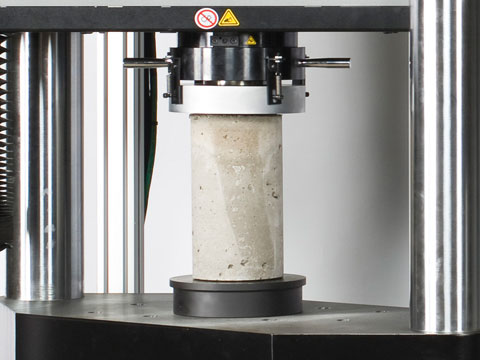
\includegraphics[scale=0.5]{imagenes/ASTM_C39_image1.jpg}
			\caption{Probeta hormigón (Autor, año)}
			\label{probetaHormigon} 
			% Label: es para realizar referencias cruzadas, 
			% notar que se escribe todo junto y sin acentos.
		\end{figure}

	La Figura \ref{probetaHormigon} Muestra ... (Explicar las figuras. Notar que la figura fue
	citada con referencia cruzada y la numeración es automática) 
	
	%% Ver video referencias cruzadas: https://www.youtube.com/watch?v=ldU2mEWAeh4


\chapter{Resultados.} 

	
	\section{Ejemplo de titulo 2.}
		
		\subsection{Ejemplo de titulo 3.}
			
			\subsubsection{Ejemplo de titulo 4 (no numerado).}

				\paragraph{Ejemplo de título 5:}

								
	\section{Discusión de resultados.}


\chapter{Conclusiones}





%%%%%%%%%%%%%%%%%%%%%%%%%%%%%%%%%%%%%%%%%%%%%%%%%%%%%%%%%%%%%%%%%%%%%%%%%%%%%%%%%%%%%%%%%%%%%%%%%
%%%%%%%%%%%%%%%%%%%%%%%%%%%%%%%%%%%% Bibliografía %%%%%%%%%%%%%%%%%%%%%%%%%%%%%%%%%%%%%%%%%%%%%%%
%%%%%%%%%%%%%%%%%%%%%%%%%%%%%%%%%%%%%%%%%%%%%%%%%%%%%%%%%%%%%%%%%%%%%%%%%%%%%%%%%%%%%%%%%%%%%%%%%
	
	% Para aprender a usar la bibliografía ver el siguiente video:
 	% https://www.youtube.com/watch?v=MnL5dI41IOA

	% No modificar esta sección
 
	\renewcommand{\refname}{Bibliografía} % Bibliografía en español
	\addcontentsline{toc}{chapter}{Bibliografía} % Agrega la bibliografía al Índice.
	\bibliographystyle{apalike} % formato APA 

	\bibliography{perifericos/bibliografia} 


%%%%%%%%%%%%%%%%%%%%%%%%%%%%%%%%%%%%%%%%%%%%%%%%%%%%%%%%%%%%%%%%%%%%%%%%%%%%%%%%%%%%%%%%%%%%%%%%%
%%%%%%%%%%%%%%%%%%%%%%%%%%%%%%%%%%%% Anexos o apéndices %%%%%%%%%%%%%%%%%%%%%%%%%%%%%%%%%%%%%%%%%
%%%%%%%%%%%%%%%%%%%%%%%%%%%%%%%%%%%%%%%%%%%%%%%%%%%%%%%%%%%%%%%%%%%%%%%%%%%%%%%%%%%%%%%%%%%%%%%%%


	% El siguiente archivo conntiene los apéndices
	% Está en un archivo diferente para que el presente archivo sea menos extenso.
	% En caso de no existir anexos simplemente eliminar o anteponer '%'
	
\appendix

\chapter{Ejemplo de apéndice o anexo}

\section{Sub título primer apéndice o anexo}



\subsection{Sub sección del primer apéndice o anexo}




\end{document}